\def\H{0.3\textwidth}
\def\W{0.7\textwidth}

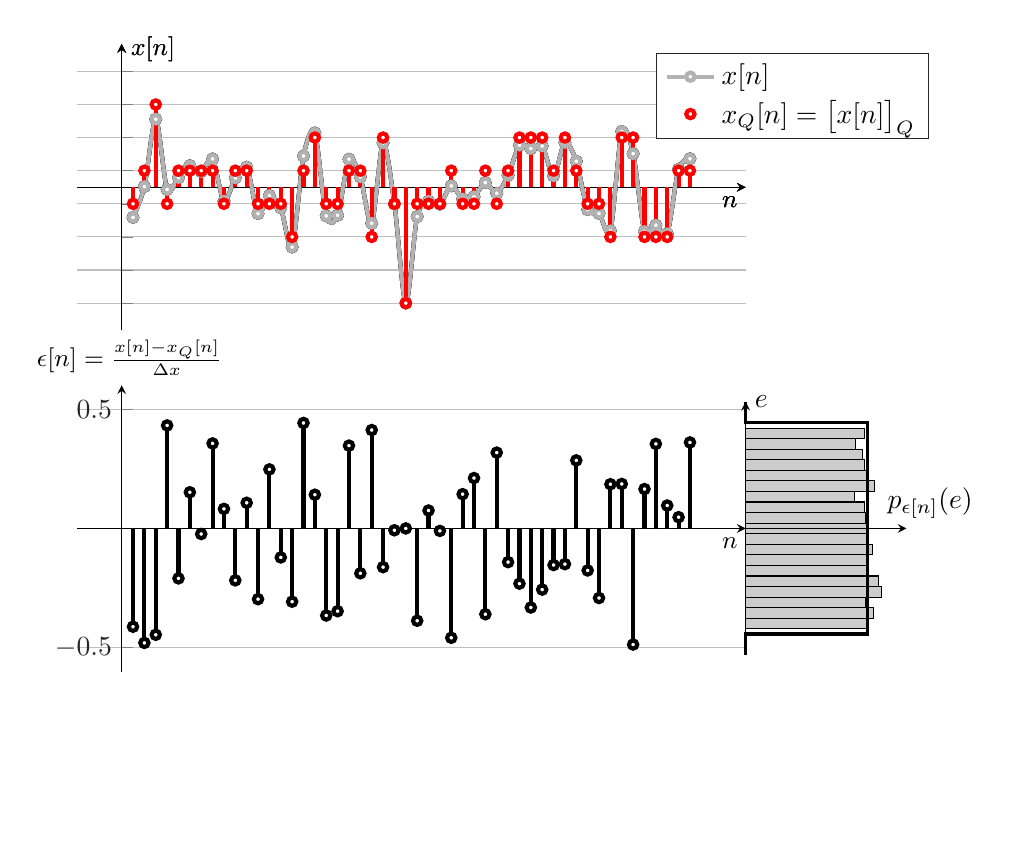
\begin{tikzpicture}
\onslide<1|handout:1>{
\begin{axis}[
name=plot1a,
axis lines*=middle,
enlargelimits = true,
width=\W,
height=\H,
clip=true,
scale only axis,
axis line style={->,>=stealth},
xlabel={\small $n$},
ylabel={\small $x[n]$},
every axis x label/.style={
	at={(ticklabel* cs:1)},
	xshift=-0.2cm,
	anchor=north,
},
every axis y label/.style={
	at={(ticklabel* cs:1)},
	xshift=0.4cm,
	yshift=-0.35cm,
	anchor=south,
},
every outer x axis line/.append style={white!15!black},
every x tick label/.append style={font=\color{white!15!black}},
xmin=1.00,
xmax=50.00,
ymin=-25.00,
ymax=25.00,
ytick=\empty,
xtick=\empty,
yticklabel=\empty,
xmajorgrids,
ymajorgrids,
every outer y axis line/.append style={white!15!black},
every y tick label/.append style={font=\color{white!15!black}},
legend style={draw=white!15!black,fill=white,legend cell align=left}]
\addplot [smooth, black, mark=*, mark options={scale=0.75, fill=white}, line width=1.5pt, forget plot]
table[row sep=crcr]{
	1 -6.3246 \\
2 0.14148 \\
3 14.2497 \\
4 -0.47482 \\
5 2.0162 \\
6 4.5187 \\
7 3.3055 \\
8 5.938 \\
9 -2.9003 \\
10 1.9589 \\
11 4.2128 \\
12 -5.5237 \\
13 -1.7526 \\
14 -4.3109 \\
15 -12.5332 \\
16 6.5333 \\
17 11.3842 \\
18 -5.9984 \\
19 -5.873 \\
20 5.874 \\
21 2.1636 \\
22 -7.5453 \\
23 9.2793 \\
24 -3.5217 \\
25 -24.2767 \\
26 -6.1509 \\
27 -2.9481 \\
28 -3.54 \\
29 0.28986 \\
30 -2.472 \\
31 -2.0041 \\
32 0.97429 \\
33 -1.2649 \\
34 2.4889 \\
35 8.7989 \\
36 8.1063 \\
37 8.627 \\
38 2.4047 \\
39 9.3665 \\
40 5.4453 \\
41 -4.6892 \\
42 -5.4897 \\
43 -9.1199 \\
44 11.6971 \\
45 7.0293 \\
46 -9.2606 \\
47 -7.9473 \\
48 -9.7386 \\
49 3.7947 \\
50 5.967 \\
};
\end{axis}
}

\onslide<2|handout:2>{
	\begin{axis}[
	name=plot1a,
	axis lines*=middle,
	enlargelimits = true,
	width=\W,
	height=\H,
	clip=true,
	scale only axis,
	axis line style={->,>=stealth},
	xlabel={\small $n$},
	ylabel={\small $x[n]$},
	every axis x label/.style={
		at={(ticklabel* cs:1)},
		xshift=-0.2cm,
		anchor=north,
	},
	every axis y label/.style={
		at={(ticklabel* cs:1)},
		xshift=0.4cm,
		yshift=-0.35cm,
		anchor=south,
	},
	every outer x axis line/.append style={white!15!black},
	every x tick label/.append style={font=\color{white!15!black}},
	xmin=1.00,
	xmax=50.00,
	ymin=-25.00,
	ymax=25.00,
	yticklabels=\empty,
	xtick=\empty,
	ytick ={-24.2767,  -17.3405,  -10.4043,   -3.4681  ,  3.4681,   10.4043,   17.3405,   24.2767},
	xmajorgrids,
	ymajorgrids,
	every outer y axis line/.append style={white!15!black},
	every y tick label/.append style={font=\color{white!15!black}},
	legend style={draw=white!15!black,fill=white,legend cell align=left}]
	\addplot [smooth, black, mark=*, mark options={scale=0.75, fill=white}, line width=1.5pt, forget plot]
	table[row sep=crcr]{
		1 -6.3246 \\
		2 0.14148 \\
		3 14.2497 \\
		4 -0.47482 \\
		5 2.0162 \\
		6 4.5187 \\
		7 3.3055 \\
		8 5.938 \\
		9 -2.9003 \\
		10 1.9589 \\
		11 4.2128 \\
		12 -5.5237 \\
		13 -1.7526 \\
		14 -4.3109 \\
		15 -12.5332 \\
		16 6.5333 \\
		17 11.3842 \\
		18 -5.9984 \\
		19 -5.873 \\
		20 5.874 \\
		21 2.1636 \\
		22 -7.5453 \\
		23 9.2793 \\
		24 -3.5217 \\
		25 -24.2767 \\
		26 -6.1509 \\
		27 -2.9481 \\
		28 -3.54 \\
		29 0.28986 \\
		30 -2.472 \\
		31 -2.0041 \\
		32 0.97429 \\
		33 -1.2649 \\
		34 2.4889 \\
		35 8.7989 \\
		36 8.1063 \\
		37 8.627 \\
		38 2.4047 \\
		39 9.3665 \\
		40 5.4453 \\
		41 -4.6892 \\
		42 -5.4897 \\
		43 -9.1199 \\
		44 11.6971 \\
		45 7.0293 \\
		46 -9.2606 \\
		47 -7.9473 \\
		48 -9.7386 \\
		49 3.7947 \\
		50 5.967 \\
	};
	\end{axis}
}

\onslide<3-|handout:3>{
\begin{axis}[
name=plot1,
axis lines*=middle,
enlargelimits = true,
width=\W,
height=\H,
clip=true,
scale only axis,
axis line style={->,>=stealth},
xlabel={\small $n$},
%ylabel={\small $x[n]$},
every axis x label/.style={
	at={(ticklabel* cs:1)},
	xshift=-0.2cm,
	anchor=north,
},
every axis y label/.style={
	at={(ticklabel* cs:1)},
	xshift=0.1cm,
	anchor=south,
},
every outer x axis line/.append style={white!15!black},
every x tick label/.append style={font=\color{white!15!black}},
xmin=1.00,
xmax=50.00,
ymin=-25.00,
ymax=25.00,
ytick ={-24.2767,  -17.3405,  -10.4043,   -3.4681  ,  3.4681,   10.4043,   17.3405,   24.2767},
xtick=\empty,
yticklabel=\empty,
xmajorgrids,
ymajorgrids,
every outer y axis line/.append style={white!15!black},
every y tick label/.append style={font=\color{white!15!black}},
legend style={draw=white!15!black,fill=white,scale=0.3,legend cell align=left, at={(axis cs: 47,10)},anchor=south west}]
\addplot [smooth, black!30, mark=*, mark options={scale=0.75, fill=white}, line width=1.5pt]
table[row sep=crcr]{
	1 -6.3246 \\
2 0.14148 \\
3 14.2497 \\
4 -0.47482 \\
5 2.0162 \\
6 4.5187 \\
7 3.3055 \\
8 5.938 \\
9 -2.9003 \\
10 1.9589 \\
11 4.2128 \\
12 -5.5237 \\
13 -1.7526 \\
14 -4.3109 \\
15 -12.5332 \\
16 6.5333 \\
17 11.3842 \\
18 -5.9984 \\
19 -5.873 \\
20 5.874 \\
21 2.1636 \\
22 -7.5453 \\
23 9.2793 \\
24 -3.5217 \\
25 -24.2767 \\
26 -6.1509 \\
27 -2.9481 \\
28 -3.54 \\
29 0.28986 \\
30 -2.472 \\
31 -2.0041 \\
32 0.97429 \\
33 -1.2649 \\
34 2.4889 \\
35 8.7989 \\
36 8.1063 \\
37 8.627 \\
38 2.4047 \\
39 9.3665 \\
40 5.4453 \\
41 -4.6892 \\
42 -5.4897 \\
43 -9.1199 \\
44 11.6971 \\
45 7.0293 \\
46 -9.2606 \\
47 -7.9473 \\
48 -9.7386 \\
49 3.7947 \\
50 5.967 \\
}; \addlegendentry{$x[n]$};

\addplot [ycomb, red, mark=*, mark options={scale=0.75, fill=white}, line width=1.5pt]
table[row sep=crcr]{
	1 -3.4681 \\
2 3.4681 \\
3 17.3405 \\
4 -3.4681 \\
5 3.4681 \\
6 3.4681 \\
7 3.4681 \\
8 3.4681 \\
9 -3.4681 \\
10 3.4681 \\
11 3.4681 \\
12 -3.4681 \\
13 -3.4681 \\
14 -3.4681 \\
15 -10.4043 \\
16 3.4681 \\
17 10.4043 \\
18 -3.4681 \\
19 -3.4681 \\
20 3.4681 \\
21 3.4681 \\
22 -10.4043 \\
23 10.4043 \\
24 -3.4681 \\
25 -24.2767 \\
26 -3.4681 \\
27 -3.4681 \\
28 -3.4681 \\
29 3.4681 \\
30 -3.4681 \\
31 -3.4681 \\
32 3.4681 \\
33 -3.4681 \\
34 3.4681 \\
35 10.4043 \\
36 10.4043 \\
37 10.4043 \\
38 3.4681 \\
39 10.4043 \\
40 3.4681 \\
41 -3.4681 \\
42 -3.4681 \\
43 -10.4043 \\
44 10.4043 \\
45 10.4043 \\
46 -10.4043 \\
47 -10.4043 \\
48 -10.4043 \\
49 3.4681 \\
50 3.4681 \\
}; \addlegendentry{$x_Q[n] = \big[x[n]\big]_Q$};
\end{axis}
}
\onslide<4-|handout:3>{
\begin{axis}[
name=plot2,
at=(plot1.below south east), anchor=above north east,
axis lines*=middle,
enlargelimits = true,
clip=true,
width=\W,
height=\H,
scale only axis,
axis line style={->,>=stealth},
xlabel={\small $n$},
ylabel={\small $\epsilon[n] = \frac{x[n]-x_Q[n]}{\Delta x}$},
every axis x label/.style={
	at={(ticklabel* cs:1)},
	xshift=-0.2cm,
	anchor=north,
},
every axis y label/.style={
	at={(ticklabel* cs:1)},
	xshift=0.1cm,
	anchor=south,
},
every outer x axis line/.append style={white!15!black},
every x tick label/.append style={font=\color{white!15!black}},
xmin=1.00,
xmax=50.00,
ymin=-0.5,
ymax=0.5,
ytick ={-0.5, 0.5},
xtick=\empty,
%yticklabel=\empty,
xmajorgrids,
ymajorgrids,
every outer y axis line/.append style={white!15!black},
every y tick label/.append style={font=\color{white!15!black}},
legend style={draw=white!15!black,fill=white,legend cell align=left}]
\addplot [ycomb, mark=*, fill=white, mark options={scale=0.75, fill=white}, line width=1.5pt, forget plot]
table[row sep=crcr]{
	1 -0.41182 \\
2 -0.4796 \\
3 -0.4456 \\
4 0.43154 \\
5 -0.20932 \\
6 0.15146 \\
7 -0.023437 \\
8 0.35608 \\
9 0.081859 \\
10 -0.21758 \\
11 0.10736 \\
12 -0.29636 \\
13 0.24732 \\
14 -0.1215 \\
15 -0.30693 \\
16 0.44191 \\
17 0.14128 \\
18 -0.3648 \\
19 -0.34672 \\
20 0.34687 \\
21 -0.18807 \\
22 0.41218 \\
23 -0.16219 \\
24 -0.0077354 \\
25 0 \\
26 -0.38678 \\
27 0.074972 \\
28 -0.01037 \\
29 -0.45821 \\
30 0.1436 \\
31 0.21106 \\
32 -0.35954 \\
33 0.31764 \\
34 -0.14117 \\
35 -0.23145 \\
36 -0.3313 \\
37 -0.25624 \\
38 -0.15331 \\
39 -0.14962 \\
40 0.28506 \\
41 -0.17604 \\
42 -0.29146 \\
43 0.18517 \\
44 0.18638 \\
45 -0.48658 \\
46 0.16489 \\
47 0.35423 \\
48 0.095976 \\
49 0.047092 \\
50 0.36027 \\
};
\end{axis}
}
\onslide<5|handout:3>{
\begin{axis}[
at=(plot2.east), %anchor=east,
anchor=origin,
%at={(1200,380)},
xmin=-0.5,
xmax=0.5,
width=1.89in,
height=1.5in,
no markers,
rotate around={-90:(current axis.origin)}, % Rotate around the origin
axis lines*=center,
every axis y label/.style={at=(current axis.above origin),anchor=south},
every axis x label/.style={at=(current axis.right of origin),anchor=west},
%height=5cm, width=8cm,
xtick=\empty,
ytick=\empty,
xticklabel=\empty,
ymin=0,
ymax=1.2,
yticklabel style = {xshift=0.4cm, yshift=-0.2cm},
ylabel=$p_{\epsilon[n]}(e)$,
xlabel={$e$},
enlargelimits=true, clip=true, axis on top,
grid = major,
axis line style={->,>=stealth},
every axis x label/.style={
	at={(ticklabel* cs:0)},
	yshift=0.2cm,
	xshift=0.2cm,
	anchor=north,
},
every axis y label/.style={
	at={(ticklabel* cs:1)},
	anchor=south,
	xshift=0.3cm,
},
x dir=reverse,
]
\addplot[black, ybar interval, fill=black!20, mark=no] plot coordinates { (-0.475000, 0.996875) (-0.425000, 1.050000) (-0.375000, 0.987500) (-0.325000, 1.112500) (-0.275000, 1.087500) (-0.225000, 1.003125) (-0.175000, 0.996875) (-0.125000, 1.043750) (-0.075000, 1.006250) (-0.025000, 1.009375) (0.025000, 0.984375) (0.075000, 0.975000) (0.125000, 0.890625) (0.175000, 1.056250) (0.225000, 0.990625) (0.275000, 0.975000) (0.325000, 0.962500) (0.375000, 0.900000) (0.425000, 0.978125) (0.475000, 0.993750) };
\addplot [very thick, black, clip=true] coordinates {(-0.6,0) (-0.5, 0) (-0.5, 1) (0.5, 1) (0.5, 0) (0.6, 0)};
\end{axis}
}
\end{tikzpicture}